\begin{figure}[centering,h]
   \begin{center}
  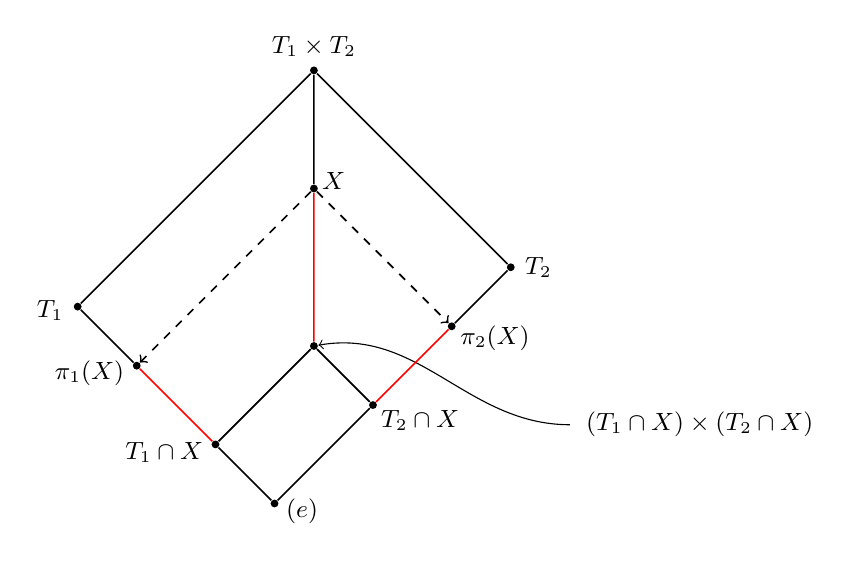
\begin{tikzpicture}[scale=.5]
    \node (e) at (0,0) [fill,circle,inner sep=1pt] {};
    \draw[font=\small] (.7,-.2) node {$(e)$};
    \node (T1capX) at (-1.5,1.5) [fill,circle,inner sep=1pt] {};
    \draw[font=\small] (-2.8,1.3) node {$T_1\cap X$};
    \node (T2capX) at (2.5,2.5) [fill,circle,inner sep=1pt] {};
    \draw[font=\small] (3.7,2.1) node {$T_2\cap X$};
    \node (pi1) at (-3.5,3.5) [fill,circle,inner sep=1pt] {};
    \draw[font=\small] (-4.7,3.3) node {$\pi_1(X)$};
    \node (pi2) at (4.5,4.5) [fill,circle,inner sep=1pt] {};
    \draw[font=\small] (5.6,4.2) node {$\pi_2(X)$};
    \node (Y) at (1,4) [fill,circle,inner sep=1pt] {};
    \draw[->] (7.5,2) to [out=180,in=10] (Y);
    \draw[font=\small] (10.8,2) node {$(T_1\cap X)\times (T_2 \cap X)$};

    \node (X) at (1,8) [fill,circle,inner sep=1pt] {};
    \draw[font=\small] (1.5,8.2) node {$X$};
    \node (T1) at (-5,5) [fill,circle,inner sep=1pt] {};
    \draw[font=\small] (-5.7,4.9) node {$T_1$};
    \node (T2) at (6,6) [fill,circle,inner sep=1pt] {};
    \draw[font=\small] (6.7,6) node {$T_2$};
    \node (T1T2) at (1,11) [fill,circle,inner sep=1pt] {};
    \draw[font=\small] (1,11.6) node {$T_1\times T_2$};


    \draw[semithick]
    (T1T2) to (X)
    (e) to (T1capX) to (Y) to (T2capX) to (e)
    (pi1) to (T1) to (T1T2) to (T2) to (pi2);

    \draw[->, dashed, semithick]
    (X) to (pi1);

    \draw[->, dashed, semithick]
    (X) to (pi2);
    
    \draw[red, semithick]
    (T1capX) to (pi1)
    (T2capX) to (pi2)
    (Y) to (X);
  \end{tikzpicture}
  \caption{Illustrates Theorem~\ref{thm:1} in case $n=2$.  Solid lines
    represent subgroup relations. Intervals colored red are isomorphic. Dashed
    lines emphasize the fact that the projections, $\pi_1(X)$ and
    $\pi_2(X)$, are not generally subgroups of $X$.}  
  \label{fig:theorem}
\end{center}
\end{figure}


